\PassOptionsToPackage{svgnames}{xcolor}
\documentclass[10pt,letterpaper]{article}
\usepackage[top=.5in, bottom=.75in, left=.5in, right=.5in]{geometry}
\usepackage{tcolorbox}
\usepackage{lipsum}
\tcbuselibrary{skins,breakable}
\usetikzlibrary{shadings,shadows}

\usepackage{graphicx} % Allows to include images
\usepackage{booktabs} % Allows the use of \toprule, \midrule and \bottomrule in tables

\usepackage{multicol}
\usepackage{float}

\usepackage[T1]{fontenc}
\usepackage[utf8]{inputenc}

\title{\vspace{-.5in}Practice 5: Focus on the Game}
\author{\vspace{-.5in}}
\date{\vspace{-.5in}}

\newenvironment{agendablock}[1]{%
    \tcolorbox[beamer,%
    noparskip,breakable,
    colback=LightGray,colframe=Black,%
    colbacklower=Gray!75!LightGray,%
    title=#1]}%
    {\endtcolorbox}

\newenvironment{evenBlock}[1]{%
    \tcolorbox[beamer,%
    noparskip,breakable,
    colback=LightGreen,colframe=DarkGreen,%
    colbacklower=LimeGreen!75!LightGreen,%
    title=#1]}%
    {\endtcolorbox}

\newenvironment{oddBlock}[1]{%
    \tcolorbox[beamer,%
    noparskip,breakable,
    colback=LightBlue,colframe=DarkBlue,%
    colbacklower=DarkBlue!75!LightBlue,%
    title=#1]}%
    {\endtcolorbox}

\newenvironment{myexampleblock}[1]{%
    \tcolorbox[beamer,%
    noparskip,breakable,
    colback=LightGreen,colframe=DarkGreen,%
    colbacklower=LimeGreen!75!LightGreen,%
    title=#1]}%
    {\endtcolorbox}

\newenvironment{myalertblock}[1]{%
    \tcolorbox[beamer,%
    noparskip,breakable,
    colback=LightCoral,colframe=DarkRed,%
    colbacklower=Tomato!75!LightCoral,%
    title=#1]}%
    {\endtcolorbox}

\newenvironment{myblock}[1]{%
    \tcolorbox[beamer,%
    noparskip,breakable,
    colback=LightBlue,colframe=DarkBlue,%
    colbacklower=DarkBlue!75!LightBlue,%
    title=#1]}%
    {\endtcolorbox}

\usepackage{lmodern}

\begin{document}
\fontfamily{lmss}\selectfont


\maketitle

\begin{agendablock}{Practice Activities}
    \begin{enumerate}
        \item Warm ups / Coerver Touches [ 15 min ]
        \item Drills [ 35 min ]
        \item Small Sided Activity [ 15 min ]
        \item Small Sided Game [ 20 min ]
        \item Sprints [ 5 min ] 
    \end{enumerate}
\end{agendablock}

\section{Warm Ups}
Run the \textbf{CLOCKS} drill until everyone arrives and for a few minutes after.

\textbf{Time: 2 minutes}
\begin{evenBlock}{Clocks (10 min)}

\begin{minipage}[t]{\linewidth}
    \centering
    
    \begin{minipage}{.3\linewidth} % Left column and width
        \centering
        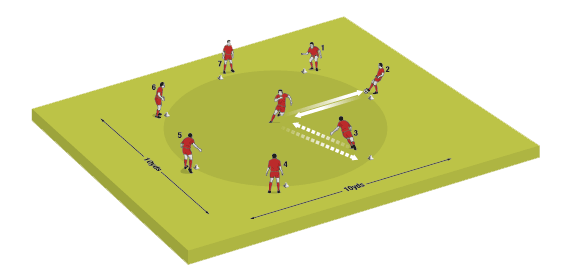
\includegraphics[width=\textwidth]{../img/Trimmed/Clocks1}
        \vspace{12pt}
        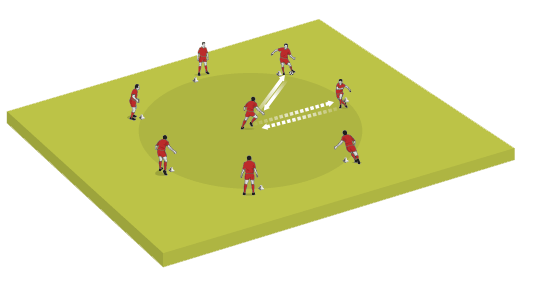
\includegraphics[width=\textwidth]{../img/Trimmed/Clocks2}
    \end{minipage}
    \hspace{0.05\linewidth}
    \begin{minipage}{.6\linewidth} % Left column and width
        \textbf{Drill Description:}
        Create a circle with your players of around 10 yards in diameter. Place cones around the circle where each player should stand, or go inside the centre circle and get the players to take a few steps forwards to get the right size. We’ve used eight players.
        \begin{enumerate}
        \setlength{\itemsep}{0pt}
        \setlength{\parskip}{0pt}
        \setlength{\parsep}{0pt}
        \item Start with the player in the middle who passes to one of the players around the circle
        \item Immediately the pass gets away, the centre player swaps position with the player clockwise from the player he passed to.
        \item The player he swaps with must get quickly into the centre to receive the ball and pass it to the next player anti-clockwise around the circle.
        \item Players continue to pass anti-clockwise and swap position with the player clockwise5. Try and get players to use one touch to get the ball around the clock
        \end{enumerate}
        
        \textbf{Coaching Points:}
        \begin{itemize}
        \setlength{\itemsep}{0pt}
        \setlength{\parskip}{0pt}
        \setlength{\parsep}{0pt}
        \item Focus on who gets your pass and then where you need to move.
        \item Attempt to complete this drill using a single touch.
        \end{itemize}

    \end{minipage}
\end{minipage}

\end{evenBlock}

\textbf{Time: 3 minutes}
\begin{myalertblock}{Theme of the Practice}
    \textbf{Elements of the Game!}

    \begin{itemize}
        \setlength{\itemsep}{0pt}
        \setlength{\parskip}{0pt}
        \setlength{\parsep}{0pt}
        \item throw-ins
        \item corner kicks - offense
        \item corner kicks - defending
        \item direct kicks - defending
        \item direct kicks - taking
        \item keeper distribution: punt, throw, goal kick.
        \item kick off.
    \end{itemize}
\end{myalertblock}

\textbf{Time: 10 minutes}
\begin{agendablock}{Captain Led Warm ups / Coerver Touches (15 min) }
    \textbf{Warmups}
    \begin{enumerate}
        \item Jog to the 18 yard line and back twice with your ball (inside cut first time, outside cut the second),
        \item Side-Step to 18 yd line and back twice,
        \item Butt Kickers to the 18 yd line and back twice,
        \item Jog Backwards to the 18 yd line and back twice.
    \end{enumerate}
    \textbf{Touches}
    \begin{enumerate}
        \item Toe-Touches (20 count alternating feet).
        \item Pull back and Push Forward (10 each foot).
        \item Side to Side or Pendulums (20 count).
        \item Triangles (10 each foot).
        \item Pullback-Behind (20 count).
    \end{enumerate}
\end{agendablock}

\clearpage



\section{Throw Ins}
\textbf{Total Time: 15 minutes}

\textbf{Time: 4 minutes}
\begin{agendablock}{HOWTO: Basic Throw In:}
\begin{itemize}
    \setlength{\itemsep}{0pt}
    \setlength{\parskip}{0pt}
    \setlength{\parsep}{0pt}
    \item Both feet must be planted during the throw.
    \item Both hands must be on the ball.
    \item Ball must travel over and behind the throwers head.
\end{itemize}
\end{agendablock}

\begin{agendablock}{HOWTO: Deep Throw In:}
\begin{itemize}
    \setlength{\itemsep}{0pt}
    \setlength{\parskip}{0pt}
    \setlength{\parsep}{0pt}
    \item For a more deeper throw in the player should advance to the line,
    \item Plant one foot and drag the other keeping it in contact with the ground.
    \item Both hands must be on the ball.
    \item Ball must travel over and behind the throwers head.
\end{itemize}
\end{agendablock}

\textbf{Time: 5 minutes}
\begin{evenBlock}{Throw-In to Feet}

    Have the boys partner up.  Have one player stand out of bounds and thrown in to the other player about 3 to 5 yards away.  The throw should be directed to the feet of the field player.  The field player should trap the ball at his feet.

\end{evenBlock}

\textbf{Time: 5 minutes}
\begin{oddBlock}{Throw-In leading field player}

    Have the boys partner up.  Have one player stand out of bounds and thrown in to the other player about 3 to 5 yards away.  The field player should be standing with his body open don field.  The throw should be directed in front of the field player. The field  player should make a first touch toward goal.
\end{oddBlock}

\section{Corner Kicks - Defense}
Explain the meanings of `far post' and `near post'.
\textbf{Time: 15 minutes}
\begin{evenBlock}{Positions}
    Mid-Field Wings: At goal posts.  Near post player positioned out of the goal to cut off that near post ball.

    Far post marker inside goal marking that edge.

    Center backs marking goal side.

    Far post Fullback and center midfielder marks goal side.

    Near post fullback marks a man.

    Center Forward Near 18 corner to cut off any passes out and ready to counter attack.
\end{evenBlock}

Once setup Coach will kick a corner for the team to handle.  Switch sides of the field.

\section{Corner Kicks - Offense}
\textbf{Time: 15 minutes}
\begin{evenBlock}{Positions}
    Forward and wing Mid-Fielders lineup at the corner of the 18 yard box.

    Near post full back takes kick.

    Center mid-fielder and Far post full back line up between near post 18 yard line and side line. Center mid runs to the PK spot, full back hovers playing the ball.

    Center backs should be at half field, keeper at his 18 yard line or further out.
    
\end{evenBlock}

\clearpage

\section{Direct Kicks - Defense}
\textbf{Time: 15 minutes}
\begin{evenBlock}{Positions}
    Form a Wall as close to the kicker as possible- center forward, mid field wing(s).  Make the referee move you away from the kick.  Center turn and face the keeper and adjust left or right as directed.   

    Defenders mark goal side within the funnel.
\end{evenBlock}

\section{Direct Kicks - Offense}
\textbf{Time: 15 minutes}
\begin{evenBlock}{Positions}
    If the ball is in the 
\end{evenBlock}

\section{Small Sided Activity}
\textbf{Time: 15 minutes, Started at 1:15 PM to 1:20 PM}

\begin{evenBlock}{Block Passing}

\begin{minipage}[t]{\linewidth}
    \centering
    
    \begin{minipage}{.4\linewidth} % Left column and width
        \centering
        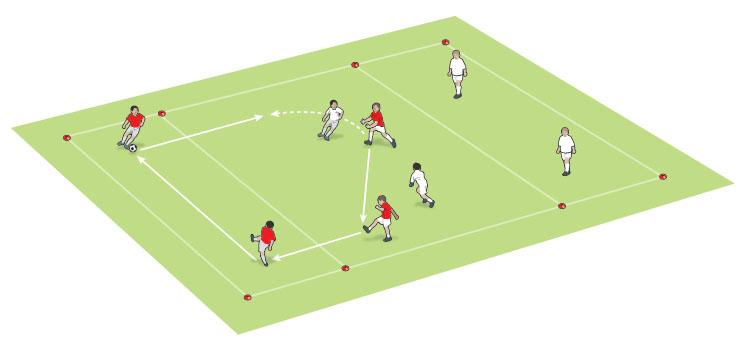
\includegraphics[width=\textwidth]{../img/Trimmed/Block_Passing_1}
        \vspace{6pt}
        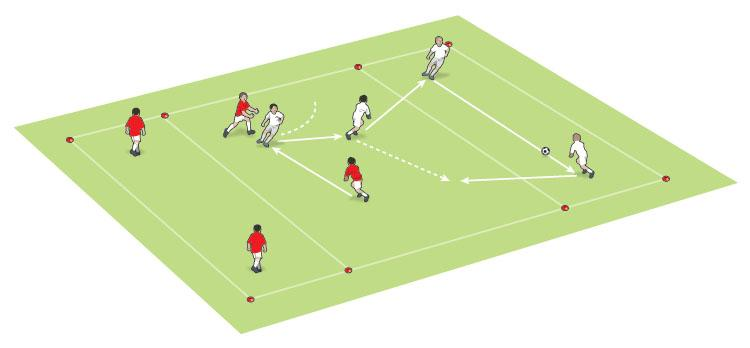
\includegraphics[width=\textwidth]{../img/Trimmed/Block_Passing_2}
    \end{minipage}
    \hspace{0.05\linewidth}
    \begin{minipage}{.5\linewidth} % Left column and width
        \textbf{Drill Description:}
        A drill that focuses on pressing and avoiding the press.  The goal is to keep the ball as long as possible.
        
        \begin{enumerate}
        \setlength{\itemsep}{0pt}
        \setlength{\parskip}{0pt}
        \setlength{\parsep}{0pt}
        \item This is a 4v4 game.
        \item 20x15 yard area with two 5 yard end zones.
        \item The end zones are safe zones and are occupied with 2 teammates.
        \item The other 2 teammates from each team are in the central zone playing 2v2 keep away.
        \item The center players can pass to the end zone players who are safe from attack, but only after they successully passed it within the central zone.
        \end{enumerate}

        \textbf{Coaching Points:}
        \begin{enumerate}
        \setlength{\itemsep}{0pt}
        \setlength{\parskip}{0pt}
        \setlength{\parsep}{0pt}
        \item Where are you passing options?
        \item Support your teammate.
        \item Know where the ball is!
        \item Block the ball or the pass.  Know where your team is.
        \item Without the ball move and talk so your partner knows where you are without seeing you.
        \end{enumerate}
    \end{minipage}
\end{minipage}

\end{evenBlock}

\section{Game}

\textbf{Start Time: 1:35 PM}

\begin{oddBlock}{Small Sided}
    \textbf{Time:} 10 minute halves.

    \textbf{Size:} 4v4 or 5v5.

    Express:
    \begin{itemize}
        \setlength{\itemsep}{0pt}
        \setlength{\parskip}{0pt}
        \setlength{\parsep}{0pt}
        \item  remind them about the practice goals and expectation there is a lot of movement and passing.
        \item Funnel Positioning.
        \item Go outside on our defensive half.
        \item Pass quickly down sidelines or into open space.
        \item Avoid passing backward.
        \item Make a pass early or move early.
    \end{itemize}

\end{oddBlock}

\section{Close}
\begin{oddBlock}{Sprints (5 min)}
    Agility runs to cone 5 yards away, stop and step circling cone then explode to next cone, circling it then explode sprinting to half field, jog back to end line and repeat 3 times.
\end{oddBlock}

\end{document}